\begin{exercises}

\exercise 远离恒星的宇宙空间充满了温度$T=2.8\si{K}$的热辐射(称为宇宙背景辐射),这是宇宙发展早期“大爆炸"的遗迹. 试估算这种“背景辐射”的光子数密度.

\exercise 在宇宙发展的早期,温度极高,热辐射光子互相碰撞,可以转变成一对正负电子.试估算当时温度的量级.

\exercise 对于光子被自由电子散射(康普锁散射)问题,设光子能量远小于$m_{e}c^{2}$,则散射过程中电子的能量、动量变化可以用牛顿力学处理.试作出相应的计算,求光的波长变化与散射角的关系.

\begin{wrapfigure}[6]{r}{10em}
	\centering
	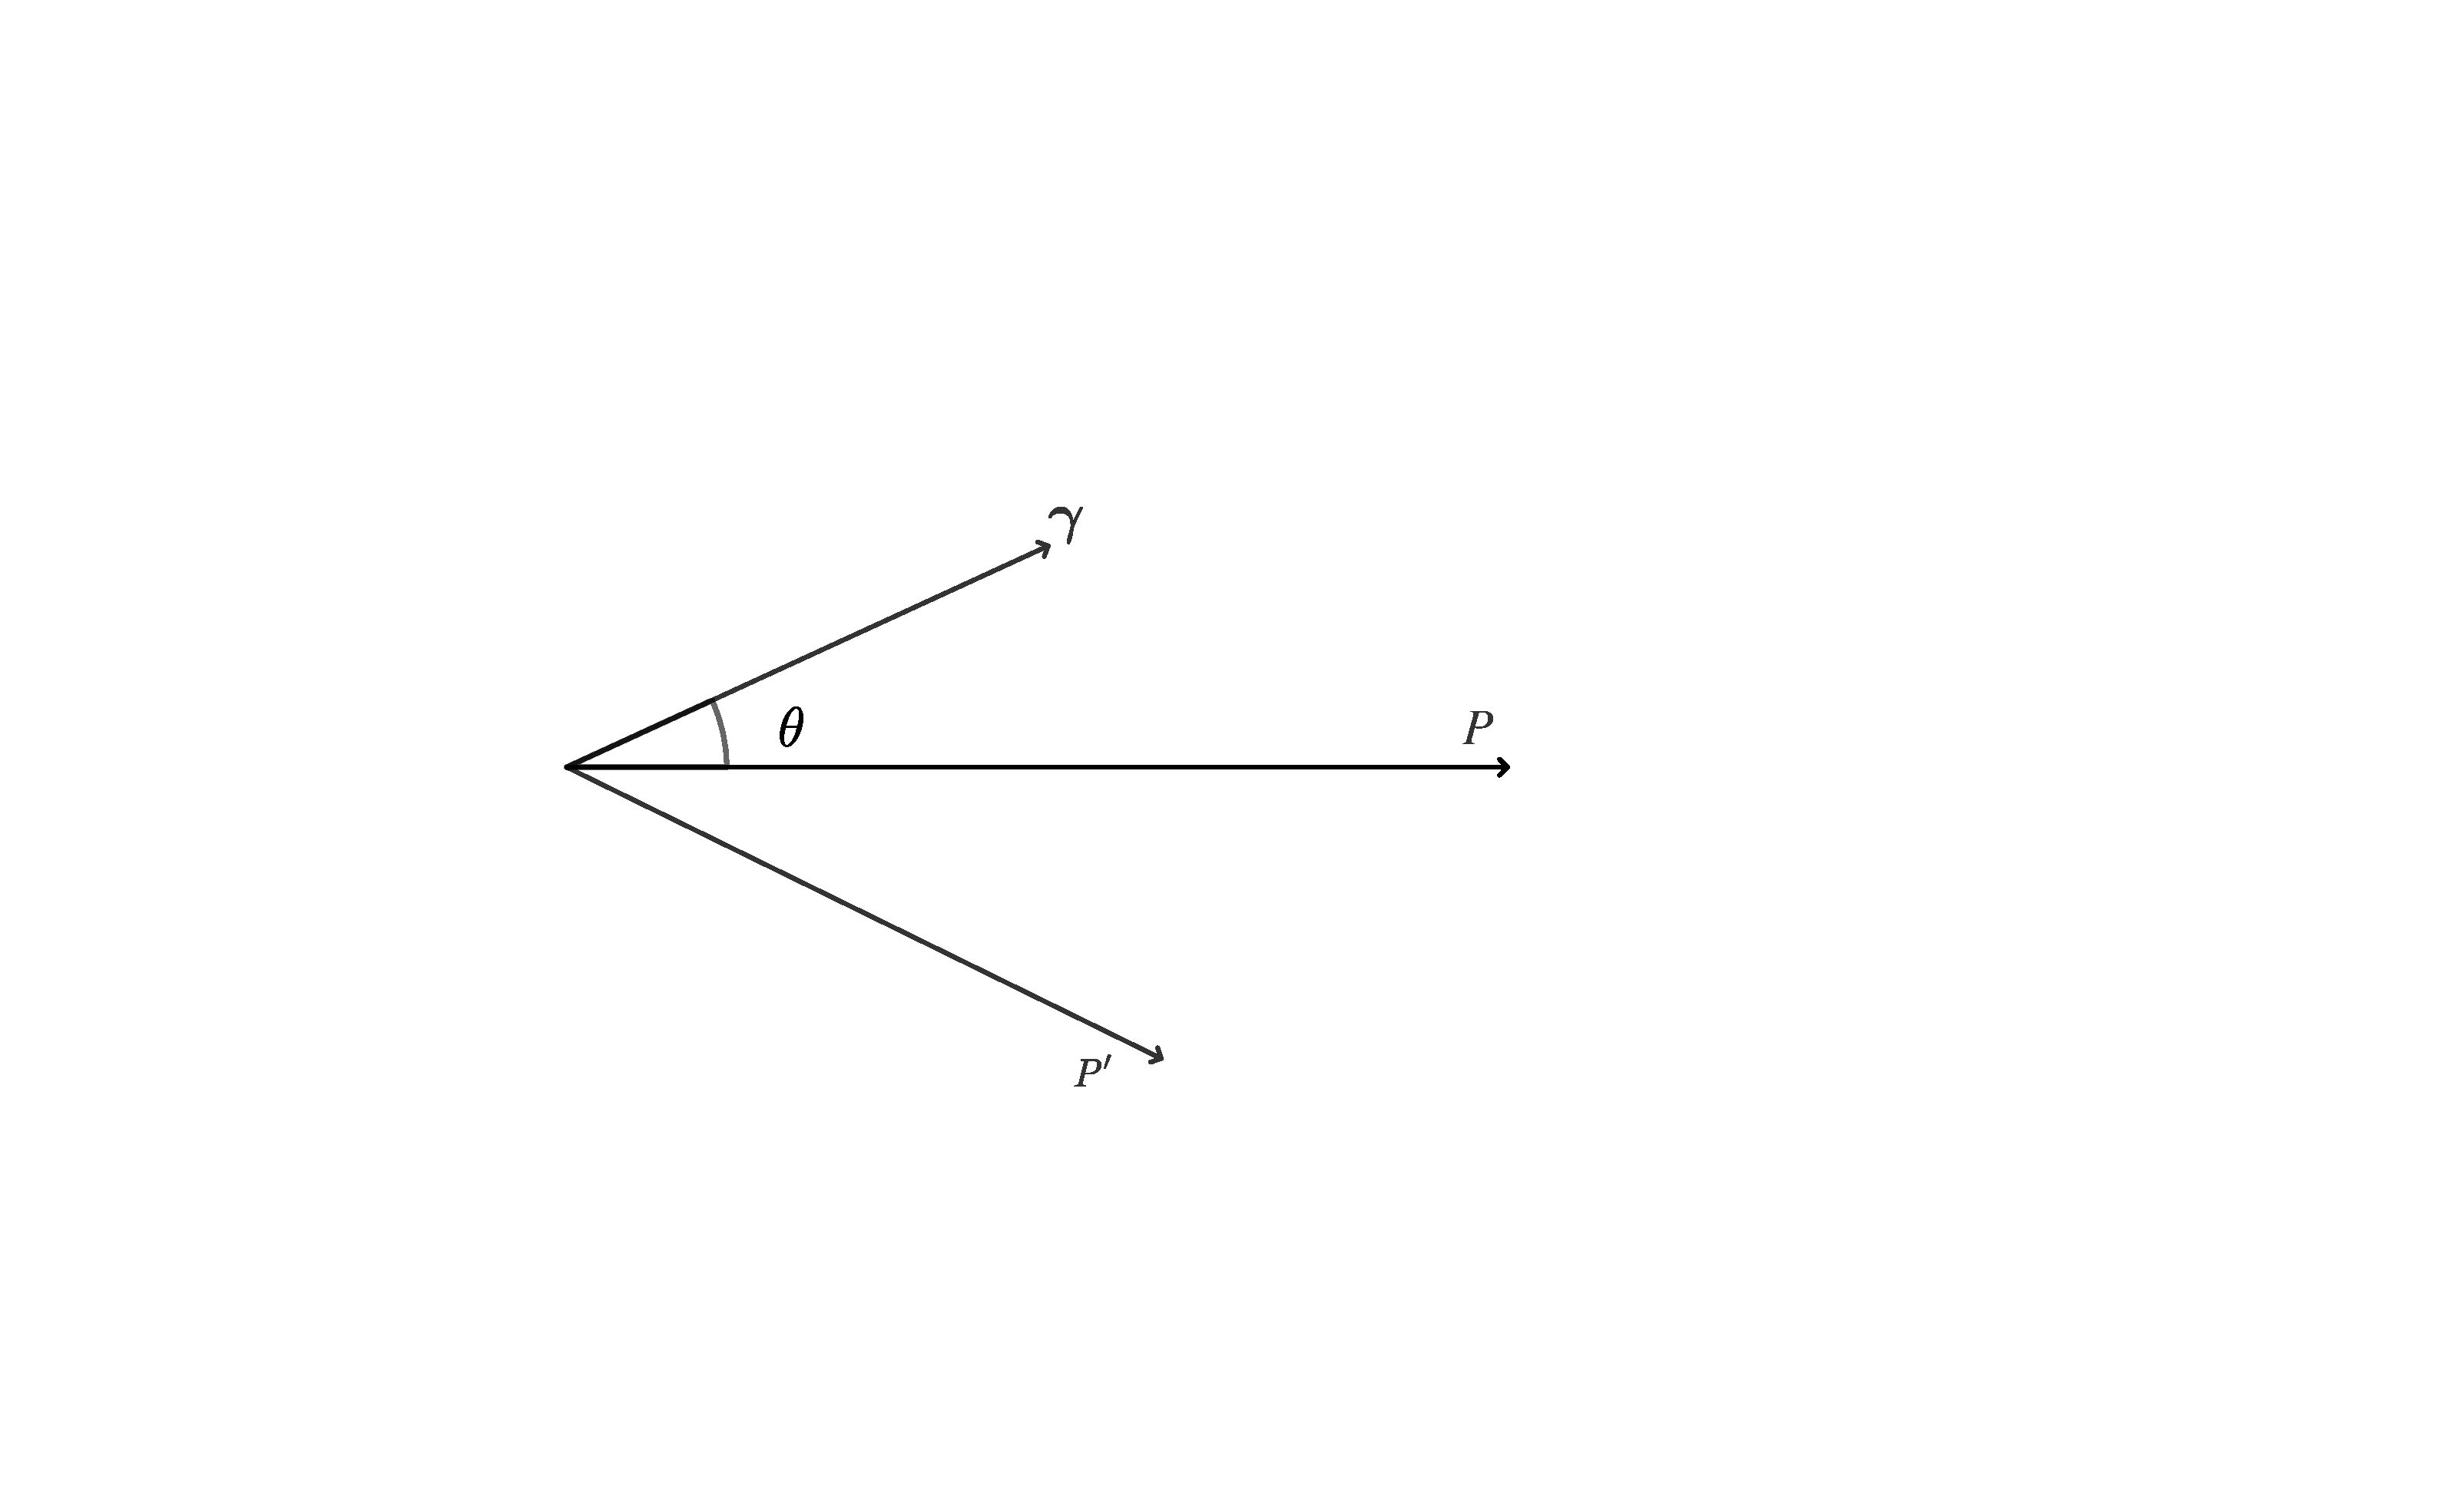
\includegraphics[width=3.5cm,clip]{QM file/figure/1-9}
	\caption{1-4题图}
	\label{fig.1-9}
\end{wrapfigure}
\exercise 高能带电粒子在介质中运动,如其速度$v$超过电磁波在介质中的传播速度,就产生切仑科夫辐射.设介质的折射率为$n$,辐射光与粒子运动方向的夹角为$\theta$.试利用光子的能量,动量公式($E_{\gamma}=\hbar\omega,p_{\gamma}=\hbar k$)以及能量守恒及动量守恒定律,求$\theta$与$n,v$的关系

$\big[\text{提示:光在介质中传播时,}\omega=\dfrac{ck}{n}. \big]$

\exercise 从质量为$m$,半径为$R$的星球表面辐射出频率为$\nu_{0}$的光,当这种光在远离星球处被观测到时,测得的频率$\nu<\nu_{0}$,这种现象称为恒星光谱的“引力红移”.设光子可以当作“质点”,引力质量$m_{\text{光}}=\dfrac{h\nu}{c^{2}}$下,光子离开星球时,必须克服星球对它的万有引力.试根据这种通俗模型导出$\dfrac{\nu}{\nu_{0}}$的公式.

\exercise 来自其他恒星的光掠过太阳(质量$M$,半径$R$)表面时,光线方向发生微小的偏转($\theta$).这个现象曾是广义相对论的实验支柱之一.试利用$1\sim 5$题中光子的“质点”模型对偏转角$\theta$作出量级估算.
\begin{figure}[!h]
	\centering
	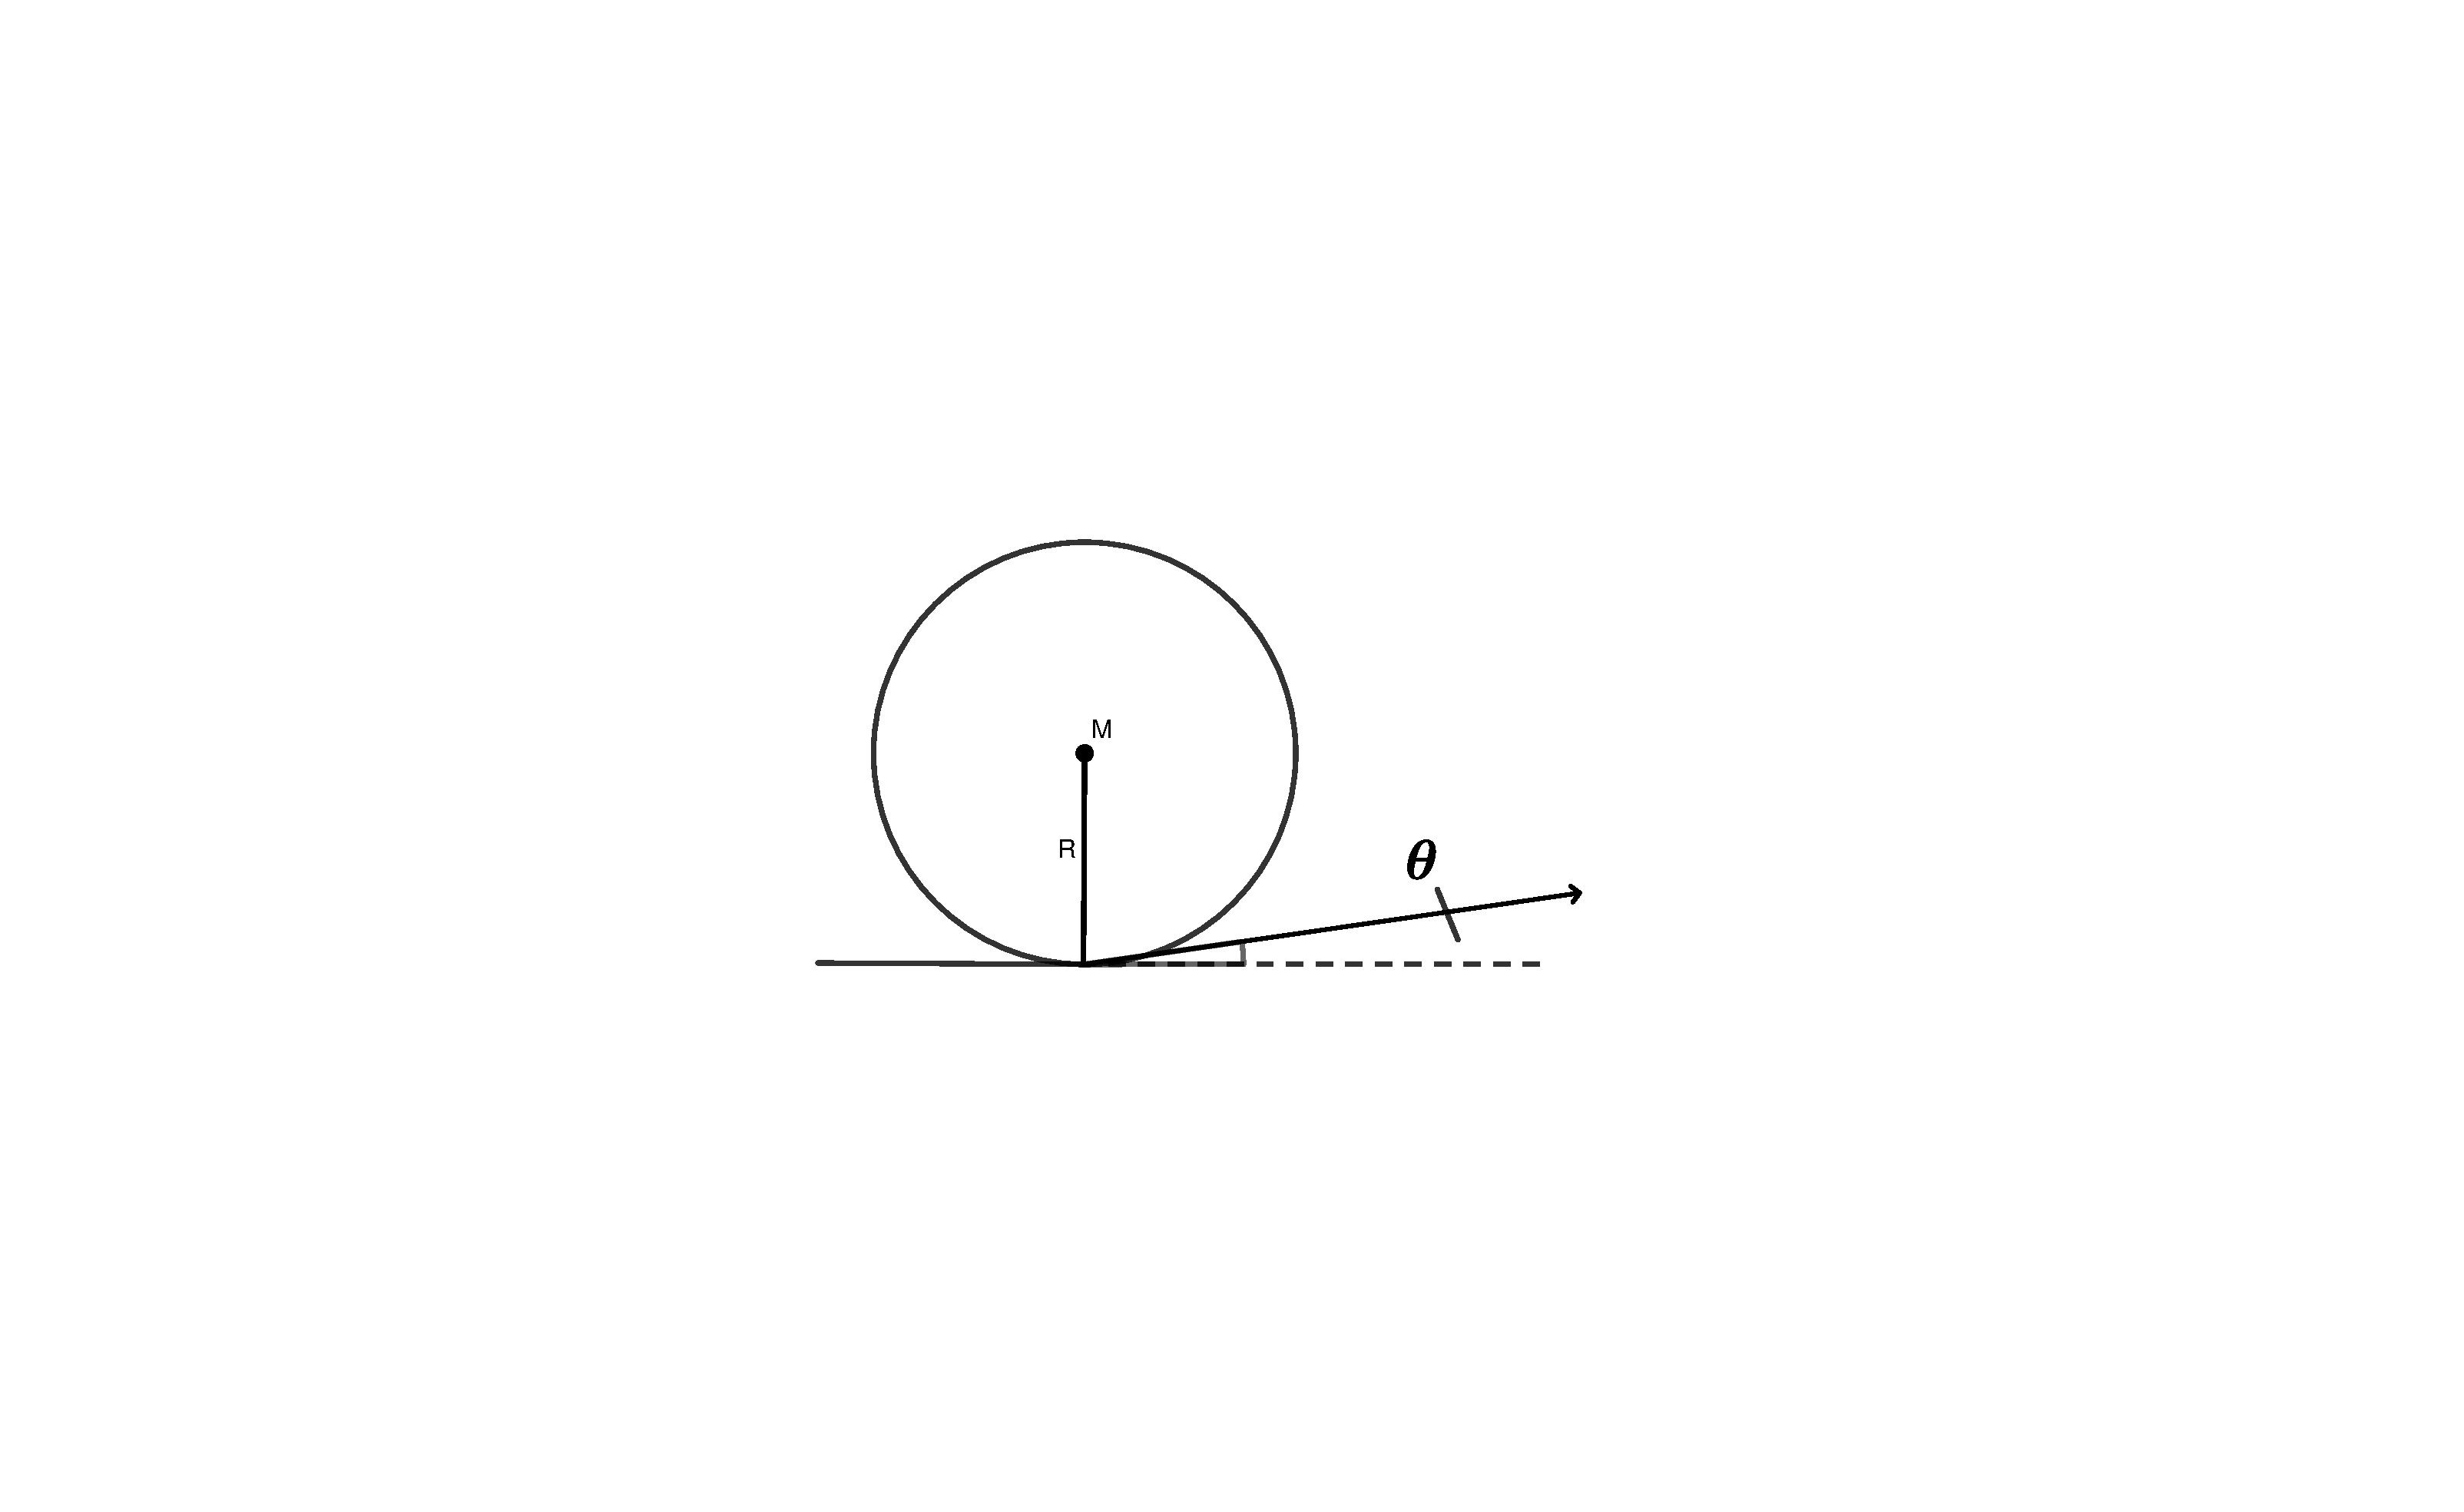
\includegraphics[width=3.5cm,clip]{QM file/figure/1-10}
	\caption{1-6题图}	\label{fig.1-10}
\end{figure}
\exercise 氢原子中电子-质子间库仑吸引力远大于万有引力.求这两种力的比率.理论上,电子与中子间的万有引力也可以使它们形成类似于氢原子的构造,试求这种“引力原子” 的基态半径公式及数值.

\exercise (a) $\mu^{-1}$子电荷为$-e$,质量$m_{\mu}=207m_{e}$,$\mu^{-1}$子与原子核(电荷$Ze$)由于库仑吸引力的作用而形成类似氢原子的构造.称为$\mu$原子.视原子核为点电荷,求$\mu$原子半径公式.
	
\quad (b) 原子核可视为电荷均匀分布的球体, 核半径的经验公式为
\begin{equation*}
	R=r_{0p}Z^{1/3},\quad r_{0p}=1.635\si{fm}
\end{equation*}
对于较大的原子序数$Z$,核半径$R$有可能大于$\mu$原子半径.求出现这种情况的$Z$的临界值$Z_{0}$. 

\exercise 计算原子核(电荷$Ze$,半径$R$)中各质子间库仑排斥能的总和及(按质子)平均值.原子核半径公式见1-8题.当$Z$取多大数值时,每个质子的平均库仑能达到核力结合能(每个核子约8\si{MeV})的量级?

\exercise 电子自旋磁矩等于$\mu_{B}$=$\dfrac{\e\hbar}{2m_{\e}c}$(玻尔磁子).在磁场$(B)$中电子获得的磁作用能大致为$B\mu_{B}$量级.如$B\mu_{B}\sim10^{-3}\si{eV}$,求磁场$B$的量级.

\exercise 估算氢分子转动能级的“解冻温度”.氢分子键长$R=0.74\times10^{-8}\si{cm}$.

\exercise 由于电磁场的真空量子效应,两块相隔距离$d$的不带电大导体平板间产生微弱吸引力设单位面积受力F,试用量纲分析法确定$F$与各基本普适常数及距离$d$的关系.

\exercise { (a) 求室温(T=300 \si{K})下中子的德布罗意波长.
	
	\quad (b) 如上述中子在地面附近垂直下落1\si{m},求波长变化的比率.
}

\exercise 如普朗克常数的值变成现有值的2倍,而其他基本常数之值不变,下列各项数值变为现有值的多少倍?

(a)原子半径 \quad (b)晶体密度 \quad (c)蓄电池的电压

\exercise 质量为$m$的粒子受弹性力$F=-kx(k>0)$作用而作一维简谐振动,按照经典力学可以求出其运动规律为
\begin{equation*}
	x(t)=A\sin(\omega t+\alpha),\quad \omega=\sqrt{\frac{k}{m}}
\end{equation*}
A为振幅谐振子的能量为$E=\dfrac{1}{2}kA^{2}$.以上请读者自行验证.试再利用玻尔-索末菲量子化条件或对应原理证明能量及振幅的量子化结果:
\begin{equation*}
	E_{n}=n\hbar\omega,\quad A_{n}=\sqrt{\frac{2n\hbar}{m\omega}},\quad n=0,1,2,\cdots
\end{equation*}
$\big[$提示:宏观的谐振动电荷,辐射的电磁波频率与振动频率相同.据此,再利用对应原理,很容易得出结论.$\big]$

\exercise 质量为$m$的粒子在大小一定的向心力$\boldsymbol{F}=-\dfrac{k\boldsymbol{r}}{r}$作用下作圆周运动.先用经典力学证明轨道半径$r$,角速度$\omega$,总能量$E$有如下关系:
\begin{equation*}
	r\omega^{2}=\frac{k}{m},\quad \boldsymbol{E}=\frac{3}{2}k\boldsymbol{r}=\frac{3}{2}\frac{k^{2}}{m\omega^{2}}
\end{equation*}
再利用量子化条件或对应原理证明能级的量子化公式:
\begin{equation*}
	E_{n}=\frac{3}{2}\bigg(\frac{\hbar^{2}k^{2}n^{2}}{m} \bigg)^{\frac{1}{3}},\quad n=1,2,3,\cdots
\end{equation*}
 
\end{exercises}